\chapter{Image Acquisition and Calibration}

As mentioned in the system architecture, images need to be taken simultaneously. There also needs to be two cameras due to the way the cameras are constructed, with a Bayer matrix for each pixel. At the time of inception, one could only isolate NIR from RGB using separate cameras. Attempts to have both on a single camera were ineffective (explain why).\\

\noindent
The

\section{Review of concepts}

\subsection{Intrinsic Parameters}

\subsubsection{Bayer matrix}

\subsection{Extrinsic Parameters}

\subsubsection{Jello effect}

\section{Filters}

The blue Rosco 2008 filter is used as in Figure \ref{fig:blue_filter}, and passes only NIR within the green and red channels, as shown in Figure \ref{fig:blue_curve}.

\begin{figure}[H]
\begin{subfigure}{0.5\textwidth}
\centering
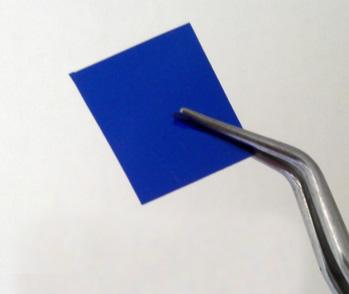
\includegraphics[scale=0.45]{images/blue_filter.jpg}
\caption{Blue Rosco 2008 filter.\\ Reproduced from \cite{blue_filter}}
\label{fig:blue_filter}
\end{subfigure}
\begin{subfigure}{0.5\textwidth}
\centering
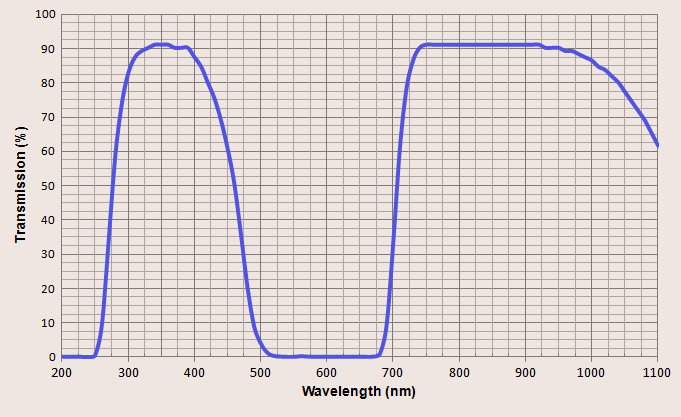
\includegraphics[scale=0.42]{images/superblueinfraredfiltercurve.png}
\caption{Blue filter transmission curve.}
\label{fig:blue_curve}
\end{subfigure}
\caption{Blue filter characteristics.\\
Reproduced from \cite{blue_curve}}
\label{fig:blue_character}
\end{figure}

\section{Camera mount}

Ripple / jello

Thus, a DC brushless motorised gimbal will not be necessary.

\section{Simultaneous triggering}

Initially TCP triggering was used, but the overhead and asynchronous nature meant that it was never consistently triggered at the same time. Instead, the clocks are sychronised using NTP, and attempt to trigger every second, on the second. The latter solution works quite well, with an occassional few milliseconds difference in stereo captures.

\section{Calibration}

Stereorectification